\section{Part I}
\subsection{One vs Rest}
The One vs Rest method to generalise a two-class classifier to a 
$k$-class classifier works by maintaining 
$k$ two-class classifier models that are trained in parallel in an online fashion. Each sub model treats the positive class as class 
$i \in \{1,\dots,k\}$ and the negative class as the set of all other classes 
$j \neq i$, hence each sub model is itself a two-class classifier that learns a linear separator between the ‘One’ target class and the ‘Rest’ (i.e. whether a point belongs to the target class or not).

Training proceeds sequentially by iterating through the data and updating the models one example at a time. For each new data point, all 
$k$ one vs rest sub models are evaluated to produce a score equivalent to how $confident$ each sub model is that the new data point belongs to its target class. Geometrically this is equivalent to quantifying how close the point is to the decision boundary associated with the model, i.e if the point is close to the decision boundary its less confident about its prediction than if the point was far away from the decision boundary. Note, scores may be positive or negative, with a large positive value indicating strong confidence that the point lies in the target class and a large negative value indicating strong confidence that it belongs to the ‘Rest’.

This process yields $k$ scores, one for each sub-model. Prediction of the global $k$ class classifier is finalised by aligning its prediction with the most 'positively confident' sub-model, the most confident being the model with the greatest positive score/confidence.

After scoring and the global prediction, each sub-model is updated immediately if its prediction (defined by the score) disagrees with the corresponding binary label for the current example. This online update process allows the classifiers to adapt incrementally as data are observed.
\subsection{One vs Rest Kernel Perceptron Implementation}
\begin{algorithm}[H]
\caption{Online One-vs-Rest Kernel Perceptron}
\begin{algorithmic}[1]

\STATE \textbf{Input:} Training data $\{(x_i,y_i)\}_{i=1}^m$, classes $\{1,\dots,K\}$, kernel $K(\cdot,\cdot)$, epochs $T$
\STATE \textbf{Initialise:} For each class $k$, set $I^{(k)}=\emptyset$, $\alpha^{(k)}=\emptyset$

\FOR{$t=1,\dots,T$}
    \FOR{$i=1,\dots,m$}
        \FOR{$k=1,\dots,K$}
            \STATE $s_k(x_i)=\sum_{j\in I^{(k)}} \alpha_j^{(k)} K(x_j,x_i)$
        \ENDFOR

        \STATE $\hat{y}=\arg\max_k s_k(x_i)$ \quad \text{(score based)}

        \FOR{$k=1,\dots,K$}
            \STATE
            $
            y_i^{(k)} =
            \begin{cases}
            +1 & \text{if } y_i = k \\
            -1 & \text{otherwise}
            \end{cases}
            $

            \IF{$\mathrm{sign}(s_k(x_i)) \neq y_i^{(k)}$}
                \STATE $I^{(k)} \leftarrow I^{(k)} \cup \{i\}$
                \STATE $\alpha^{(k)} \leftarrow \alpha^{(k)} \cup y_i^{(k)}$
            \ENDIF
        \ENDFOR
    \ENDFOR
\ENDFOR

\end{algorithmic}
\end{algorithm}

To determine a suitable number of training epochs, we first investigated the convergence pattern of the OvR kernel perceptron algorithm. Initially the model was trained over 20 independent runs using 1-30 epochs, and the average train and test error was recorded. The resulting accuracy curves showed rapid convergence, with both training and test accuracy plateauing after a small number of epochs. The model was then again trained over 20 independent runs but an early stopping criteria was implemented. Upon completing each epoch pass the model was validated on a 10\% validation subset that was held out from the training data. Training was terminated when the improvement in validation accuracy failed to improve by a tolerance of $10^{-3}$ for 3 epochs in a row.

\begin{figure}[H]
    \centering

    \begin{subfigure}{0.48\textwidth}
        \centering
        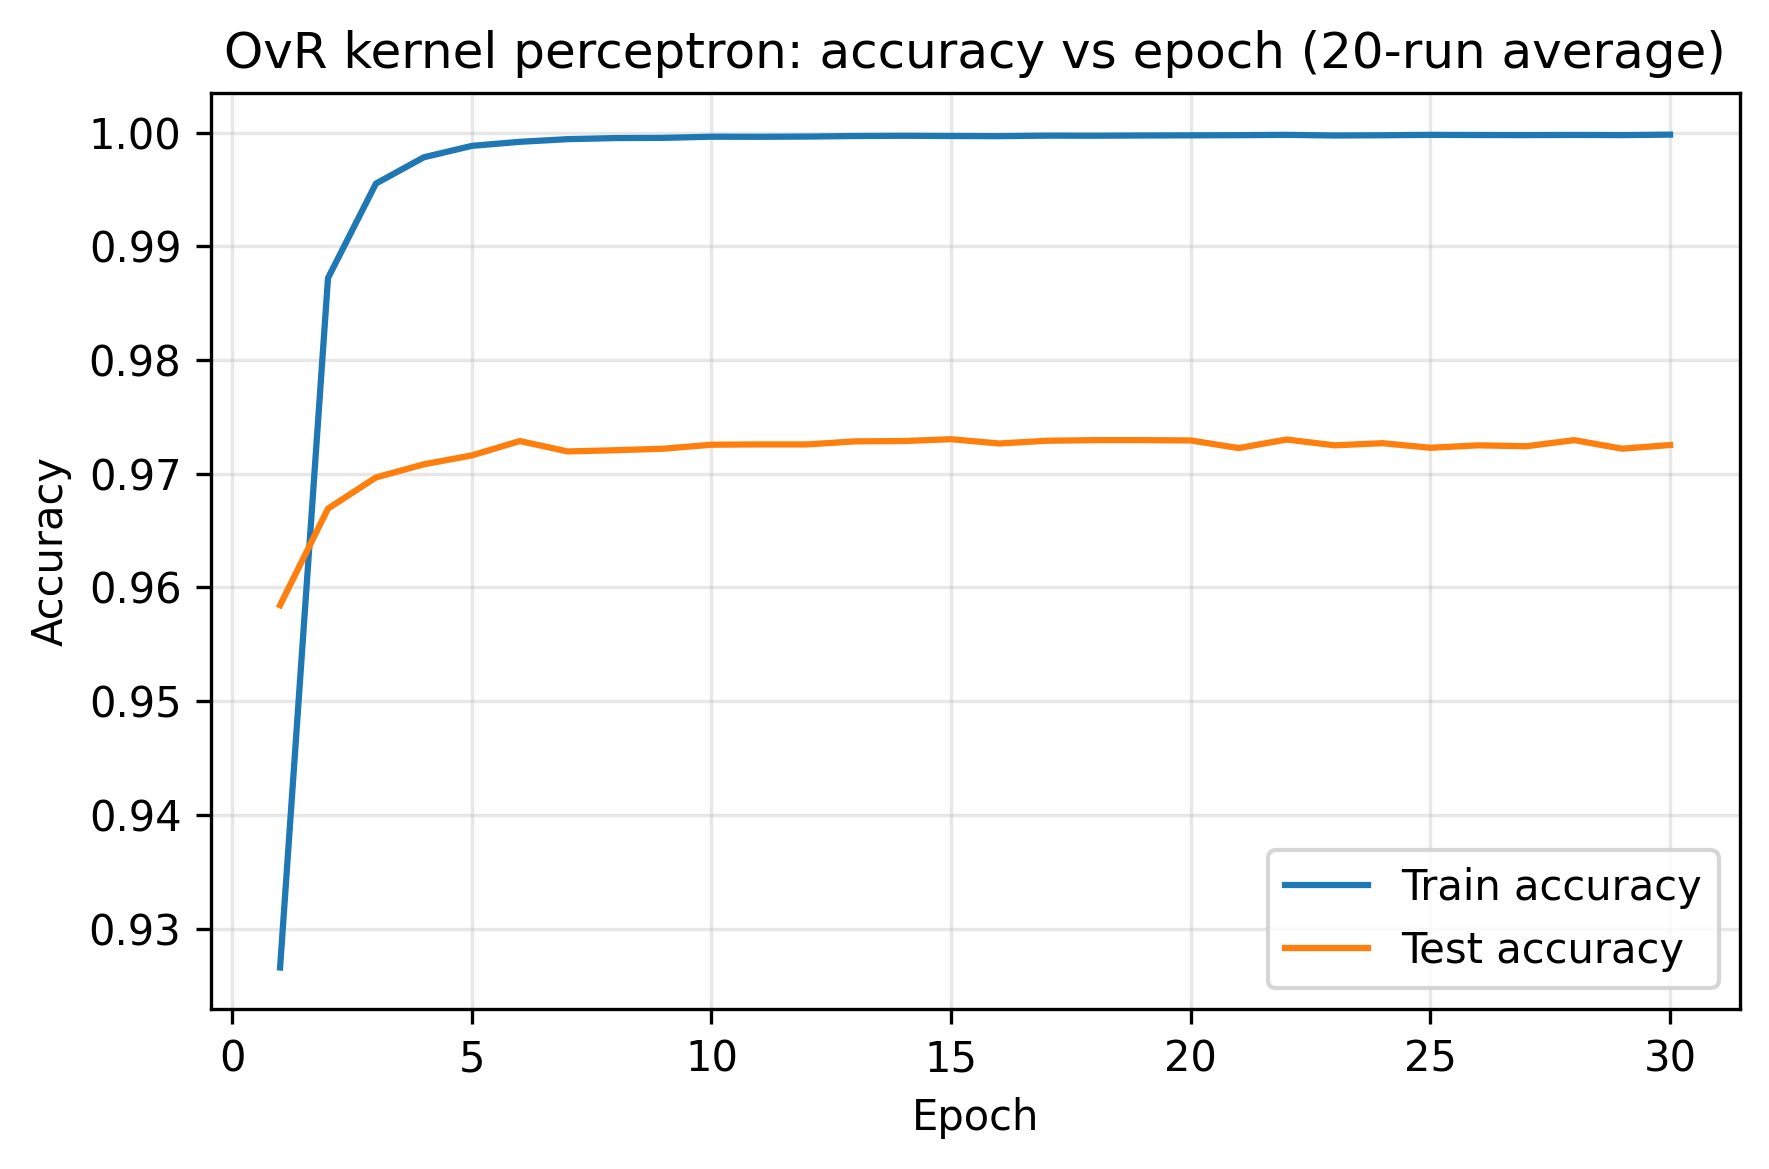
\includegraphics[width=\textwidth]{outputs/figures/OvR_poly_epoch_diagnostic_avg_accuracy_vs_epoch.png}
        \caption{}
    \end{subfigure}
    \hfill
    \begin{subfigure}{0.48\textwidth}
        \centering
        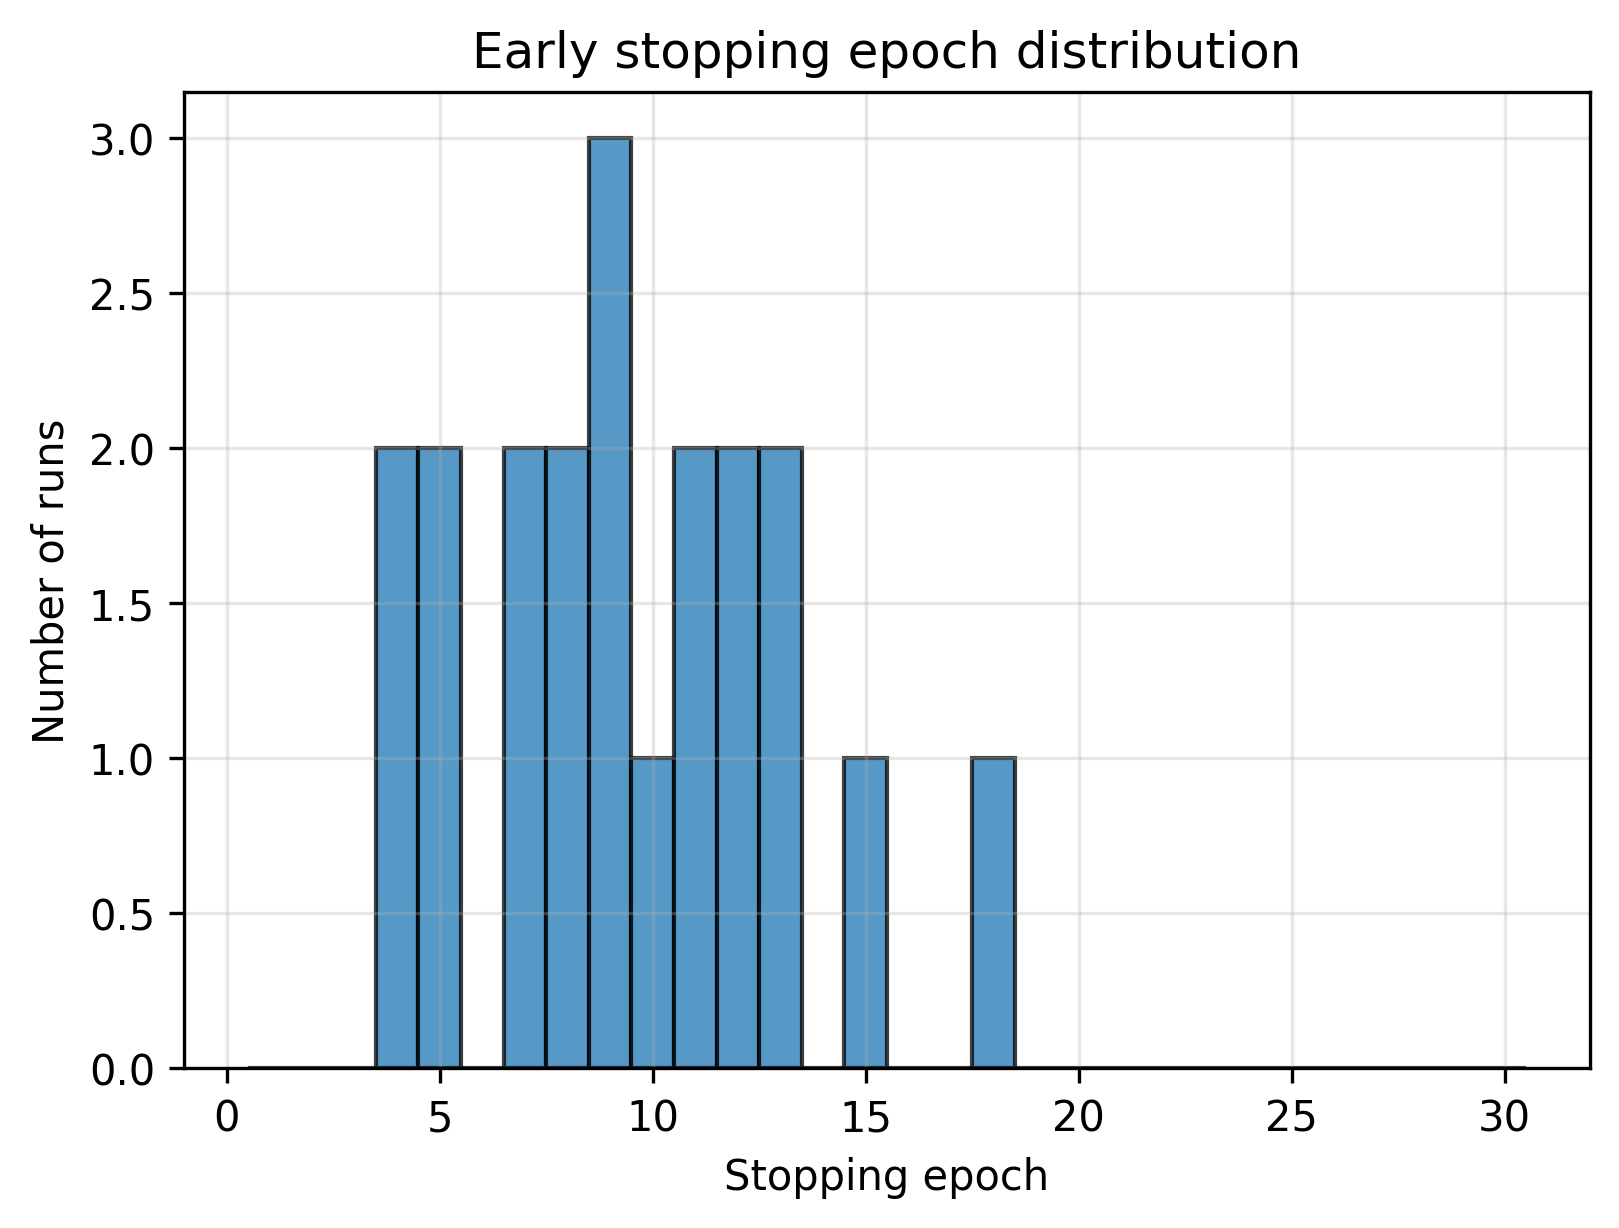
\includegraphics[width=\textwidth]{outputs/figures/OvR_epoch_diagnostic_stopping_epochs copy.png}
        \caption{}
    \end{subfigure}
\end{figure}

The distribution of stopping epochs across runs concentrated primarily between approximately 4 and 13 epochs. Based on this analysis, number of epochs was fixed at 5 for all later experiments. This choice captures the vast majority of meaningful learning across runs whilst also avoiding unnecessary computation beyond the point of meaningful improvements. It also ensures consistency and comparability across models and results in later experiments.\\\\




\subsection{One vs Rest : Polynomial Kernel Perceptron}
We first investigate the use of a polynomial kernel.
\begin{equation}
K(p,q) = (p \cdot q)^d
\end{equation}

\subsubsection{Basic Results}
The perceptron was trained on a 80-20\% train-test split using a polynomial kernel of degree $d = 1 ... 7$. We performed 20 runs (each with a different train-test split) and evaluated the trained model on both the training set and the test set. The resulting errors were then averaged across all 20 runs and the mean and std recorded below.
\begin{table}[H]
    \centering
    \begin{tabular}{rll}
\toprule
d & mean train error rates (\%) & mean test error rates (\%) \\
\midrule
1 & 9.043 $\pm$ 0.572 & 11.882 $\pm$ 2.239 \\
2 & 3.249 $\pm$ 0.186 & 8.208 $\pm$ 1.316 \\
3 & 2.512 $\pm$ 0.28 & 7.401 $\pm$ 2.296 \\
4 & 2.347 $\pm$ 0.229 & 7.688 $\pm$ 1.801 \\
5 & 2.472 $\pm$ 0.335 & 7.491 $\pm$ 1.092 \\
6 & 2.465 $\pm$ 0.323 & 7.258 $\pm$ 1.537 \\
7 & 2.613 $\pm$ 0.397 & 7.778 $\pm$ 1.416 \\
\bottomrule
\end{tabular}

    \caption{}
    \label{tab:q2_mse}
\end{table}
The results show that as the degree of the polynomial increases, the training error decreases, this is to be expected as the more complex the model the better it becomes at fitting the training data. The test errors however tell a different story. Initially at lower polynomial degree, test errors behave similar to the train errors, low degree fits poorly and increasing the degree decreases the error. This only applies up until a point, $d = 6$, where increasing the degree beyond this point actually causes the test error to increase again, this behaviour is characteristic of overfitting as the model starts to fit the noise rather than the actual patterns in the data.\\
We can conclude that the optimal degree is $d=6$


\subsubsection{Cross-Validation}
To select the optimal polynomial degree we performed 20 runs of model fitting, this time each run included 5-fold cross validation for each polynomial degree to select the optimal parameter (degree) followed by retraining the model using the optimal parameter ($d^*$). The model was then again evaluated on the training set and the test set the results of which are listed below.
\begin{table}[H]
    \centering
    \begin{tabular}{rrr}
\toprule
run & d* & test error rate (\%) \\
\midrule
1 & 4.0000 & 12.9045 \\
2 & 4.0000 & 12.3495 \\
3 & 2.0000 & 13.9712 \\
4 & 3.0000 & 14.2631 \\
5 & 5.0000 & 14.5225 \\
6 & 5.0000 & 11.8378 \\
7 & 2.0000 & 12.3532 \\
8 & 2.0000 & 12.8973 \\
9 & 2.0000 & 13.4595 \\
10 & 6.0000 & 11.8306 \\
11 & 3.0000 & 12.9117 \\
12 & 4.0000 & 14.2486 \\
13 & 5.0000 & 10.4865 \\
14 & 5.0000 & 10.2342 \\
15 & 6.0000 & 11.5423 \\
16 & 3.0000 & 14.2631 \\
17 & 2.0000 & 13.7045 \\
18 & 6.0000 & 15.6036 \\
19 & 3.0000 & 10.7459 \\
20 & 4.0000 & 12.0829 \\
\bottomrule
\end{tabular}

    \caption{}
    \label{tab:q2_mse}
\end{table}
The results show that the optimal parameter has mean of 5.15±0.96307, train errors have a mean of 0.0511±0.037\% and test errors have a mean of 2.712±0.316\%.
This aligns with the previous results without cross-validation where we identified the optimal parameter as being $d=6$, as 6 is within the mean+std of the cross validation result.

\subsubsection{Confusion Matrix}
A confusion matrix was also computed at the same time as cross-validation. The results were averaged across 20 runs and they show us the rate which the model confused 2 labels. I.e if the true
label was “7” and “2” was predicted then the confusion error for “(7,2)” would increase.
\begin{table}[H]
    \centering
    \resizebox{\textwidth}{!}{%
        \begingroup
\scriptsize
\setlength{\tabcolsep}{3pt}
\begin{tabular}{lllllllllll}
\toprule
 & \textbf{0} & \textbf{1} & \textbf{2} & \textbf{3} & \textbf{4} & \textbf{5} & \textbf{6} & \textbf{7} & \textbf{8} & \textbf{9} \\
  &  &  &  &  &  &  &  &  &  &  \\
\midrule
0 & 0.000 ± 0.000 & 0.049 ± 0.117 & 0.145 ± 0.217 & 0.257 ± 0.219 & 0.112 ± 0.153 & 0.257 ± 0.239 & 0.274 ± 0.310 & 0.048 ± 0.151 & 0.081 ± 0.177 & 0.065 ± 0.131 \\
1 & 0.021 ± 0.092 & 0.000 ± 0.000 & 0.039 ± 0.118 & 0.019 ± 0.081 & 0.196 ± 0.314 & 0.000 ± 0.000 & 0.252 ± 0.222 & 0.039 ± 0.116 & 0.095 ± 0.164 & 0.000 ± 0.000 \\
2 & 0.248 ± 0.332 & 0.228 ± 0.337 & 0.000 ± 0.000 & 0.532 ± 0.600 & 0.762 ± 0.535 & 0.133 ± 0.231 & 0.190 ± 0.304 & 0.543 ± 0.426 & 0.457 ± 0.558 & 0.050 ± 0.151 \\
3 & 0.069 ± 0.208 & 0.120 ± 0.301 & 0.742 ± 0.663 & 0.000 ± 0.000 & 0.000 ± 0.000 & 1.600 ± 1.258 & 0.000 ± 0.000 & 0.439 ± 0.519 & 0.970 ± 0.864 & 0.216 ± 0.498 \\
4 & 0.060 ± 0.181 & 0.553 ± 0.502 & 0.614 ± 0.433 & 0.086 ± 0.205 & 0.000 ± 0.000 & 0.173 ± 0.265 & 0.545 ± 0.667 & 0.342 ± 0.452 & 0.061 ± 0.267 & 0.465 ± 0.436 \\
5 & 0.933 ± 0.981 & 0.101 ± 0.320 & 0.380 ± 0.466 & 1.075 ± 0.866 & 0.312 ± 0.405 & 0.000 ± 0.000 & 0.769 ± 0.386 & 0.102 ± 0.243 & 0.421 ± 0.573 & 0.412 ± 0.509 \\
6 & 0.922 ± 0.765 & 0.245 ± 0.359 & 0.181 ± 0.414 & 0.000 ± 0.000 & 0.383 ± 0.528 & 0.337 ± 0.460 & 0.000 ± 0.000 & 0.000 ± 0.000 & 0.178 ± 0.272 & 0.031 ± 0.136 \\
7 & 0.028 ± 0.124 & 0.239 ± 0.352 & 0.338 ± 0.532 & 0.219 ± 0.363 & 0.670 ± 0.562 & 0.132 ± 0.339 & 0.000 ± 0.000 & 0.000 ± 0.000 & 0.435 ± 0.483 & 0.856 ± 0.620 \\
8 & 0.829 ± 0.753 & 0.504 ± 0.511 & 0.360 ± 0.431 & 0.969 ± 0.891 & 0.426 ± 0.677 & 0.897 ± 0.758 & 0.310 ± 0.451 & 0.237 ± 0.530 & 0.000 ± 0.000 & 0.142 ± 0.285 \\
9 & 0.152 ± 0.263 & 0.030 ± 0.130 & 0.119 ± 0.239 & 0.158 ± 0.275 & 1.012 ± 0.733 & 0.000 ± 0.000 & 0.000 ± 0.000 & 0.846 ± 0.860 & 0.124 ± 0.248 & 0.000 ± 0.000 \\
\bottomrule
\end{tabular}

\endgroup

    }
    \caption{}
    \label{tab:q5_confusion}
\end{table}
From the confusion matrix we can see that the model struggles at telling apart digits that look very similar, such as 8 and 3, 7 and 9, 5 and 6. We can also see that it does very well at telling apart digits that dont look similar at all.
\\

\subsubsection{Hard to Predict Samples}
\begin{figure}[H]
    \centering
    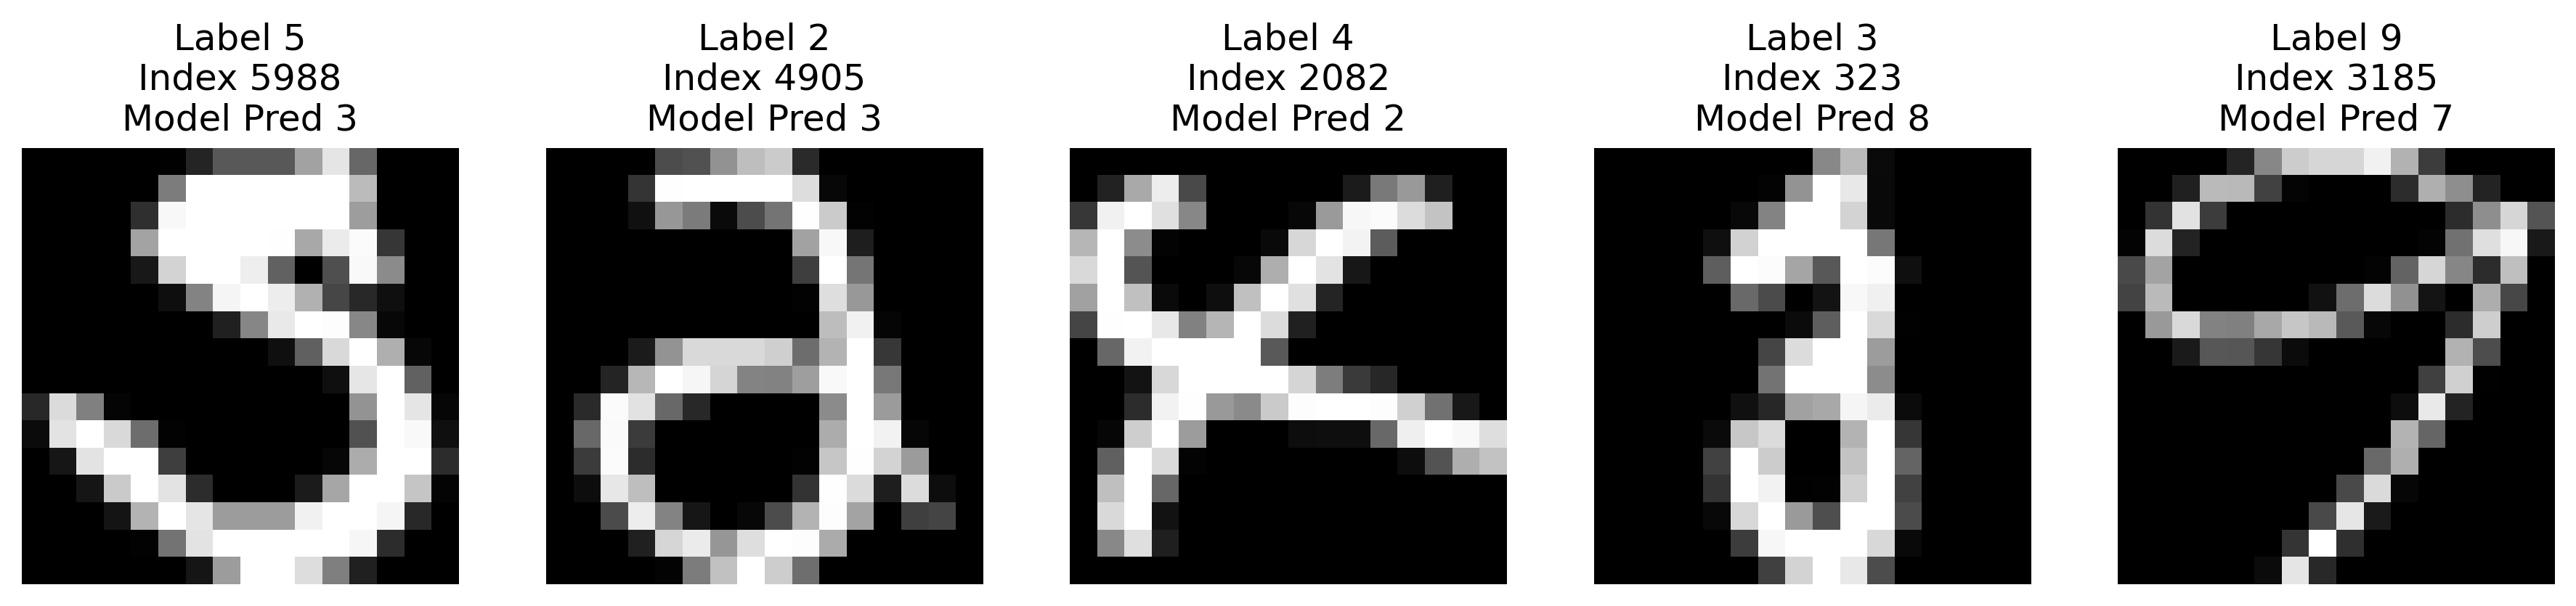
\includegraphics[width=0.7\textwidth]{outputs/figures/OvR_poly_Q6_hard_examples.png}
    \caption{}
    \label{fig:q1_poly_fits}
\end{figure}
These samples are hard to predict as they are ambiguous, take the first image for example, it has an additional stroke that makes it look like a 6 even to the human eye when in reality its labeled as a 1. The 4th image is labeled as a 0 but is distorted and the final image is labeled as an 8 but the way its been drawn within the image it looks like a 4 is present. These are all examples where the images are ambiguous and so geometrically would sit very close to the decision boundary, hence the model is more likely to incorrectly predict their labels and hence are hard to predict.
\subsection{One vs Rest: Gaussian Kernel Perceptron}
We now investigate the use of a gaussian kernel instead of a polynomial kernel.
\begin{equation}
K(p,q) = \exp\!\left(-c\,\lVert p - q \rVert^2\right)
\end{equation}

\subsubsection{Parameter selection}
To determine a suitable set $S$ of candidate values for the Gaussian kernel parameter $c$, we conducted a series of exploratory experiments on a 15\% subset of the full dataset. We first trained the model over a wide range of $c$ values in order to identify the approximate scale at which the test error was minimised. This was followed by progressively restricting the range and adopting the form $c = 2^{-b/2}$. This allowed us to focus on the region of best performance while keeping computational cost low. Finally, the most promising range of $c$ values was evaluated on the full dataset to confirm that the observed behaviour applied to the full dataset and not just the subset. Based on these experiments the final set $S$ was chosen as
\[
S = \left\{ 2^{-b/2} \;\middle|\; b \in \{9,10,\dots,15\} \right\},
\]

\begin{figure}[H]
    \centering

    \begin{subfigure}{0.48\textwidth}
        \centering
        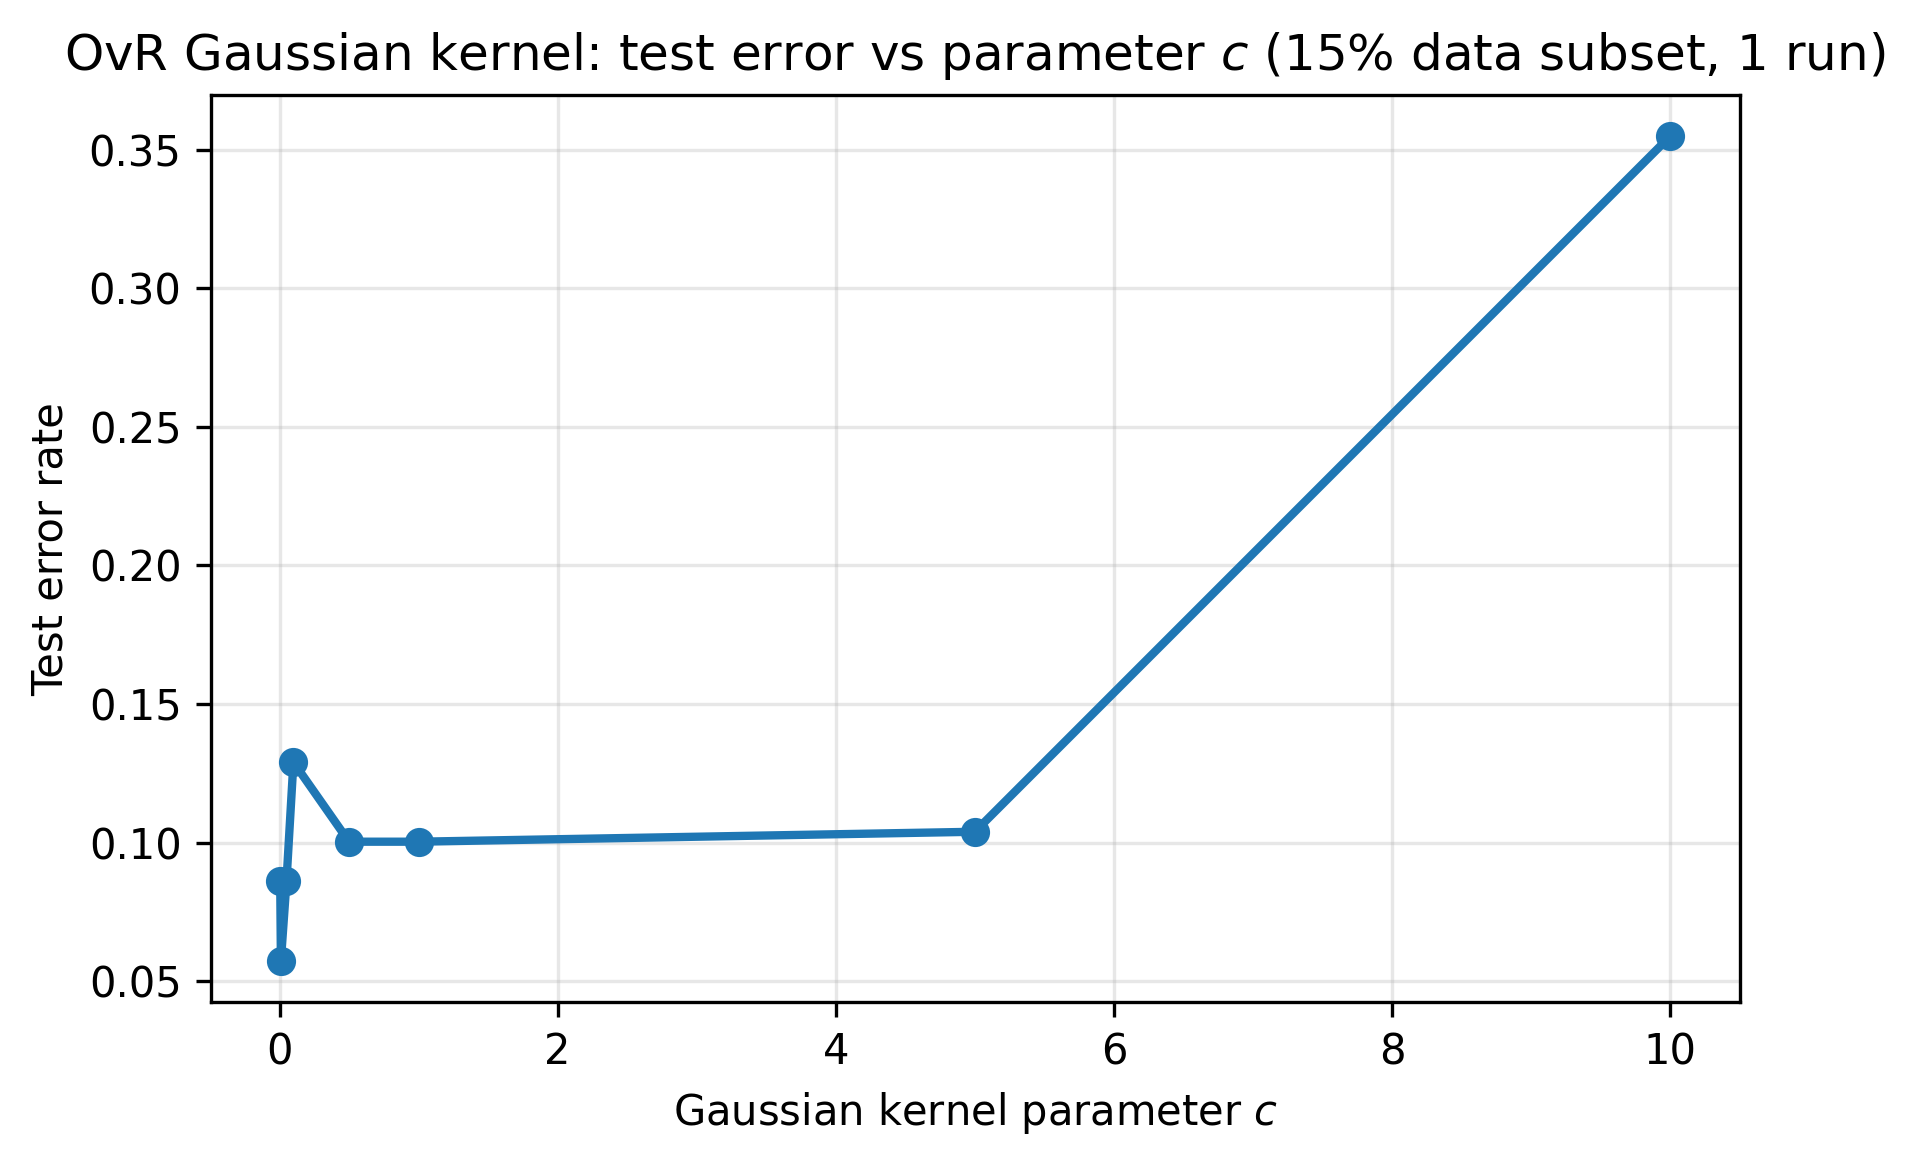
\includegraphics[width=\textwidth]{outputs/figures/Q7a_ovr_gauss_wide_15pct_param_sweep.png}
        \caption{c = [0.005, 0.01, 0.05, 0.1, 0.5, 1, 5, 10] on 15\% of the dataset}
    \end{subfigure}
    \hfill
    \begin{subfigure}{0.48\textwidth}
        \centering
        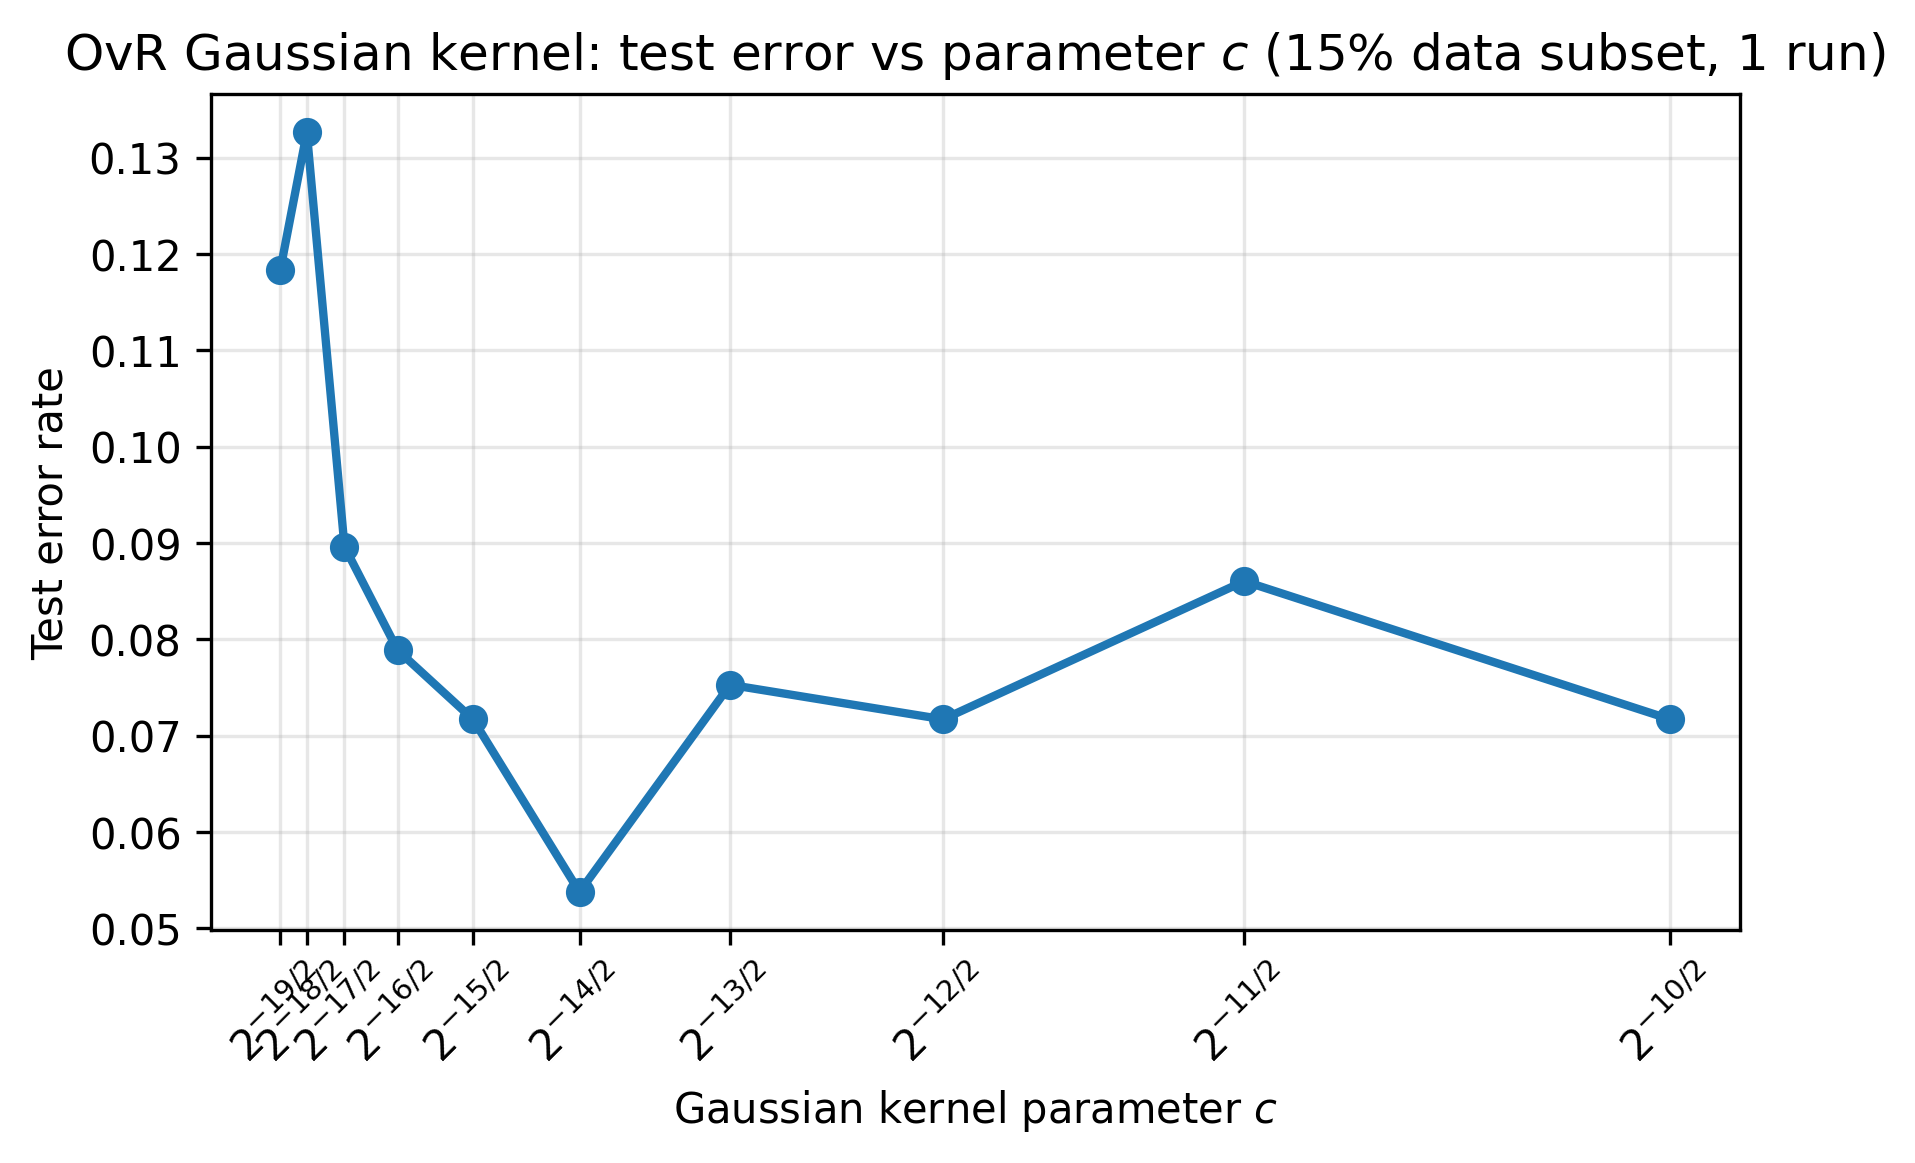
\includegraphics[width=\textwidth]{outputs/figures/Q7a_ovr_gauss_logfine_15pct_param_sweep.png}
        \caption{c = [2$^{-b/2}$, $b \in [10,20)$] on 15\% of the dataset}
    \end{subfigure}

    \vspace{0.5em}

    \begin{subfigure}{0.48\textwidth}
        \centering
        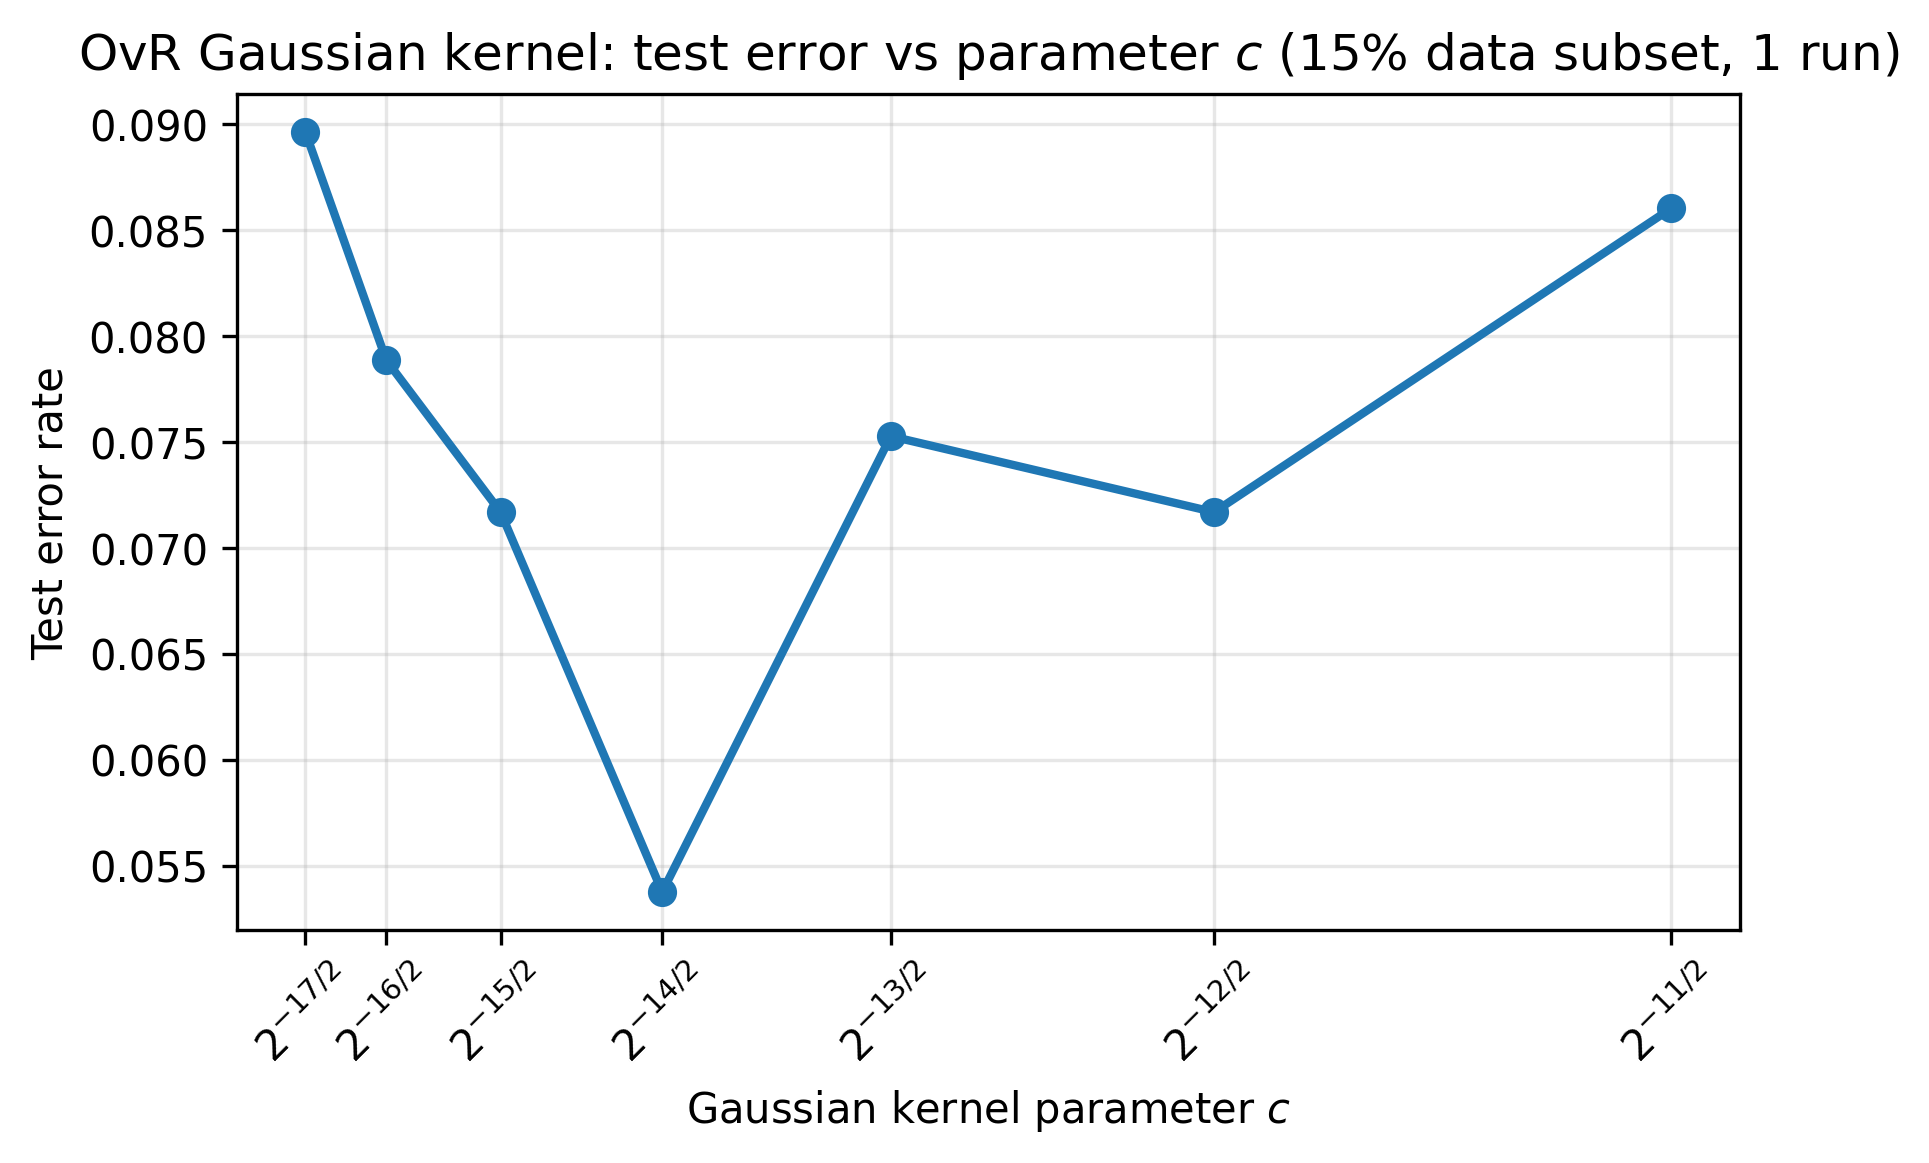
\includegraphics[width=\textwidth]{outputs/figures/Q7a_ovr_gauss_logfiner_15pct_param_sweep.png}
        \caption{c = [2$^{-b/2}$, $b \in [11,18)$] on 15\% of the dataset}
    \end{subfigure}
    \hfill
    \begin{subfigure}{0.48\textwidth}
        \centering
        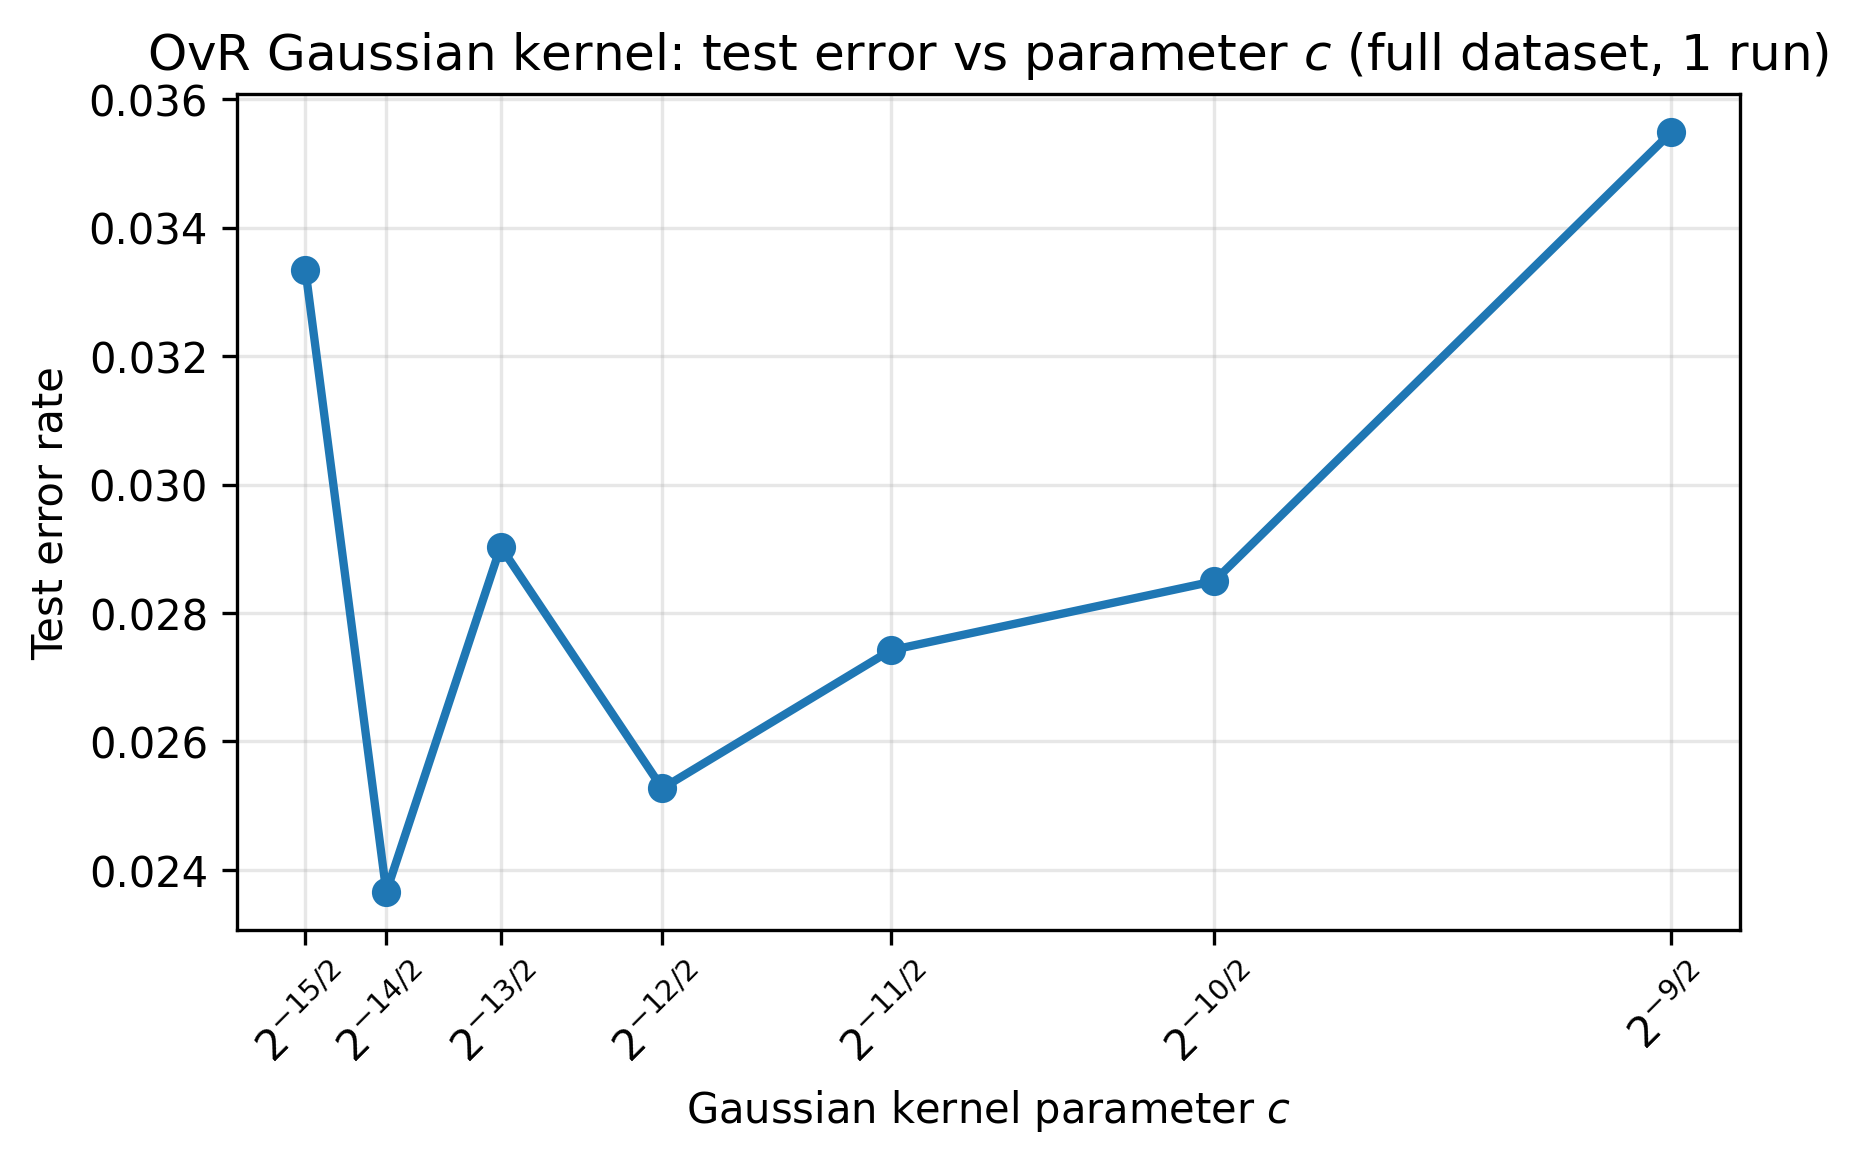
\includegraphics[width=\textwidth]{outputs/figures/Q7a_ovr_gauss_logfiner_full_param_sweep.png}
        \caption{c = [2$^{-b/2}$, $b \in [9,16)$] on full dataset}
    \end{subfigure}

    \caption{Gaussian OVR parameter sweeps at different resolutions and dataset sizes}
    \label{fig:q7a_gauss_param_sweep}
\end{figure}

\subsubsection{Basic Results}
\begin{table}[H]
    \centering
    \begin{tabular}{lll}
\toprule
c & mean train error rates (\%) & mean test error rates (\%) \\
\midrule
$2^{-9/2}$ & 2.506 $\pm$ 0.293 & 9.427 $\pm$ 1.745 \\
$2^{-10/2}$ & 2.534 $\pm$ 0.357 & 8.118 $\pm$ 1.347 \\
$2^{-11/2}$ & 2.38 $\pm$ 0.345 & 7.258 $\pm$ 1.883 \\
$2^{-12/2}$ & 2.463 $\pm$ 0.312 & 6.792 $\pm$ 1.713 \\
$2^{-13/2}$ & 2.592 $\pm$ 0.348 & 6.989 $\pm$ 1.808 \\
$2^{-14/2}$ & 2.564 $\pm$ 0.3 & 6.953 $\pm$ 1.462 \\
$2^{-15/2}$ & 2.885 $\pm$ 0.17 & 7.025 $\pm$ 1.656 \\
\bottomrule
\end{tabular}

    \caption{}
    \label{tab:q2_mse}
\end{table}
From the results above we observe the expected U shape in test errors, as the value of $c$ decreases the test errors initially decrease up until the point $c = 2^{-12/2}$, after which decreasing $c$ further causes test errors to increase. An interesting observation to note is that unlike in the polynomial case where training errors continued to decrease as $c$ decreased, in the gaussian case the training errors also exhibited a U shape like the test errors. This is because in the with the gaussian kernel the width parameter defines locally the influence of training points are. If the width is too small, the model doesn't effectively capture the similarity between points, if its too wide data points too far away influence the model too strongly. Hence the extremes cause poor performance in both the test and training errors.

We conclude that the optimal parameter is $c=2^{-12/2}$
\subsubsection{Cross Validation}
\begin{table}[H]
    \centering
    \begin{tabular}{rrr}
\toprule
run & c* & test error rate (\%) \\
\midrule
1 & 0.0110 & 2.8637 \\
2 & 0.0156 & 3.1459 \\
3 & 0.0156 & 3.0788 \\
4 & 0.0110 & 2.7024 \\
5 & 0.0110 & 2.8504 \\
6 & 0.0110 & 2.6889 \\
7 & 0.0110 & 2.6351 \\
8 & 0.0156 & 2.8099 \\
9 & 0.0110 & 2.6889 \\
10 & 0.0078 & 2.7560 \\
11 & 0.0221 & 2.5813 \\
12 & 0.0156 & 2.6486 \\
13 & 0.0156 & 2.9175 \\
14 & 0.0156 & 2.5007 \\
15 & 0.0110 & 2.8636 \\
16 & 0.0156 & 2.8368 \\
17 & 0.0156 & 2.8098 \\
18 & 0.0156 & 2.6217 \\
19 & 0.0156 & 2.7964 \\
20 & 0.0156 & 2.8099 \\
\bottomrule
\end{tabular}

    \caption{}
    \label{tab:q2_mse}
\end{table}
The results show that the optimal parameter has mean of 0.01575±0.0037037 = $2^{-11.97700872/2}$±0.0037037, train errors have a mean of 0.0336±0.0183\% and test errors have a mean of 2.5242±0.3927\%.
This aligns with the previous results without cross-validation where we identified the optimal parameter as being $c=2^{-12/2}$
\subsubsection{Confusion error matrix}
\begin{table}[H]
    \centering
    \resizebox{\textwidth}{!}{%
        \begingroup
\scriptsize
\setlength{\tabcolsep}{3pt}
\begin{tabular}{lllllllllll}
\toprule
 & \textbf{0} & \textbf{1} & \textbf{2} & \textbf{3} & \textbf{4} & \textbf{5} & \textbf{6} & \textbf{7} & \textbf{8} & \textbf{9} \\
  &  &  &  &  &  &  &  &  &  &  \\
\midrule
0 & 0.000 ± 0.000 & 0.000 ± 0.000 & 0.333 ± 1.453 & 0.000 ± 0.000 & 0.000 ± 0.000 & 0.294 ± 1.282 & 0.596 ± 1.803 & 0.000 ± 0.000 & 0.000 ± 0.000 & 0.000 ± 0.000 \\
1 & 0.000 ± 0.000 & 0.000 ± 0.000 & 0.000 ± 0.000 & 0.749 ± 2.303 & 1.145 ± 2.756 & 0.000 ± 0.000 & 0.000 ± 0.000 & 0.000 ± 0.000 & 0.000 ± 0.000 & 0.000 ± 0.000 \\
2 & 0.385 ± 1.676 & 1.658 ± 3.351 & 0.000 ± 0.000 & 0.357 ± 1.557 & 2.821 ± 5.431 & 1.607 ± 5.587 & 0.417 ± 1.816 & 2.683 ± 5.937 & 0.417 ± 1.816 & 0.885 ± 2.679 \\
3 & 0.625 ± 2.724 & 0.000 ± 0.000 & 1.288 ± 4.045 & 0.000 ± 0.000 & 1.339 ± 4.028 & 11.748 ± 14.243 & 0.000 ± 0.000 & 2.984 ± 5.448 & 2.583 ± 5.276 & 0.000 ± 0.000 \\
4 & 0.455 ± 1.981 & 6.117 ± 8.591 & 1.413 ± 3.425 & 1.000 ± 4.359 & 0.000 ± 0.000 & 0.556 ± 2.422 & 0.000 ± 0.000 & 1.270 ± 3.842 & 0.913 ± 2.809 & 4.574 ± 6.006 \\
5 & 2.548 ± 6.132 & 1.635 ± 3.930 & 1.458 ± 4.424 & 4.239 ± 8.848 & 1.705 ± 4.105 & 0.000 ± 0.000 & 9.837 ± 9.516 & 0.000 ± 0.000 & 0.500 ± 2.179 & 0.556 ± 2.422 \\
6 & 4.733 ± 8.009 & 1.599 ± 3.950 & 2.181 ± 4.385 & 0.000 ± 0.000 & 6.816 ± 9.177 & 1.214 ± 3.705 & 0.000 ± 0.000 & 0.000 ± 0.000 & 0.500 ± 2.179 & 0.500 ± 2.179 \\
7 & 0.000 ± 0.000 & 0.625 ± 2.724 & 0.714 ± 3.113 & 0.000 ± 0.000 & 3.806 ± 7.276 & 0.000 ± 0.000 & 1.843 ± 4.560 & 0.000 ± 0.000 & 0.000 ± 0.000 & 2.633 ± 6.829 \\
8 & 0.000 ± 0.000 & 0.833 ± 3.632 & 2.917 ± 8.849 & 5.000 ± 10.341 & 0.000 ± 0.000 & 0.714 ± 3.113 & 6.667 ± 13.333 & 0.000 ± 0.000 & 0.000 ± 0.000 & 4.583 ± 11.016 \\
9 & 2.444 ± 6.132 & 0.774 ± 2.329 & 0.000 ± 0.000 & 0.871 ± 2.616 & 2.683 ± 5.937 & 1.190 ± 3.876 & 0.000 ± 0.000 & 4.395 ± 8.621 & 1.566 ± 3.745 & 0.000 ± 0.000 \\
\bottomrule
\end{tabular}

\endgroup

    }
    \caption{}
    \label{tab:q5_confusion}
\end{table}
\subsubsection{Hard to Predict Samples}
\begin{figure}[H]
    \centering
    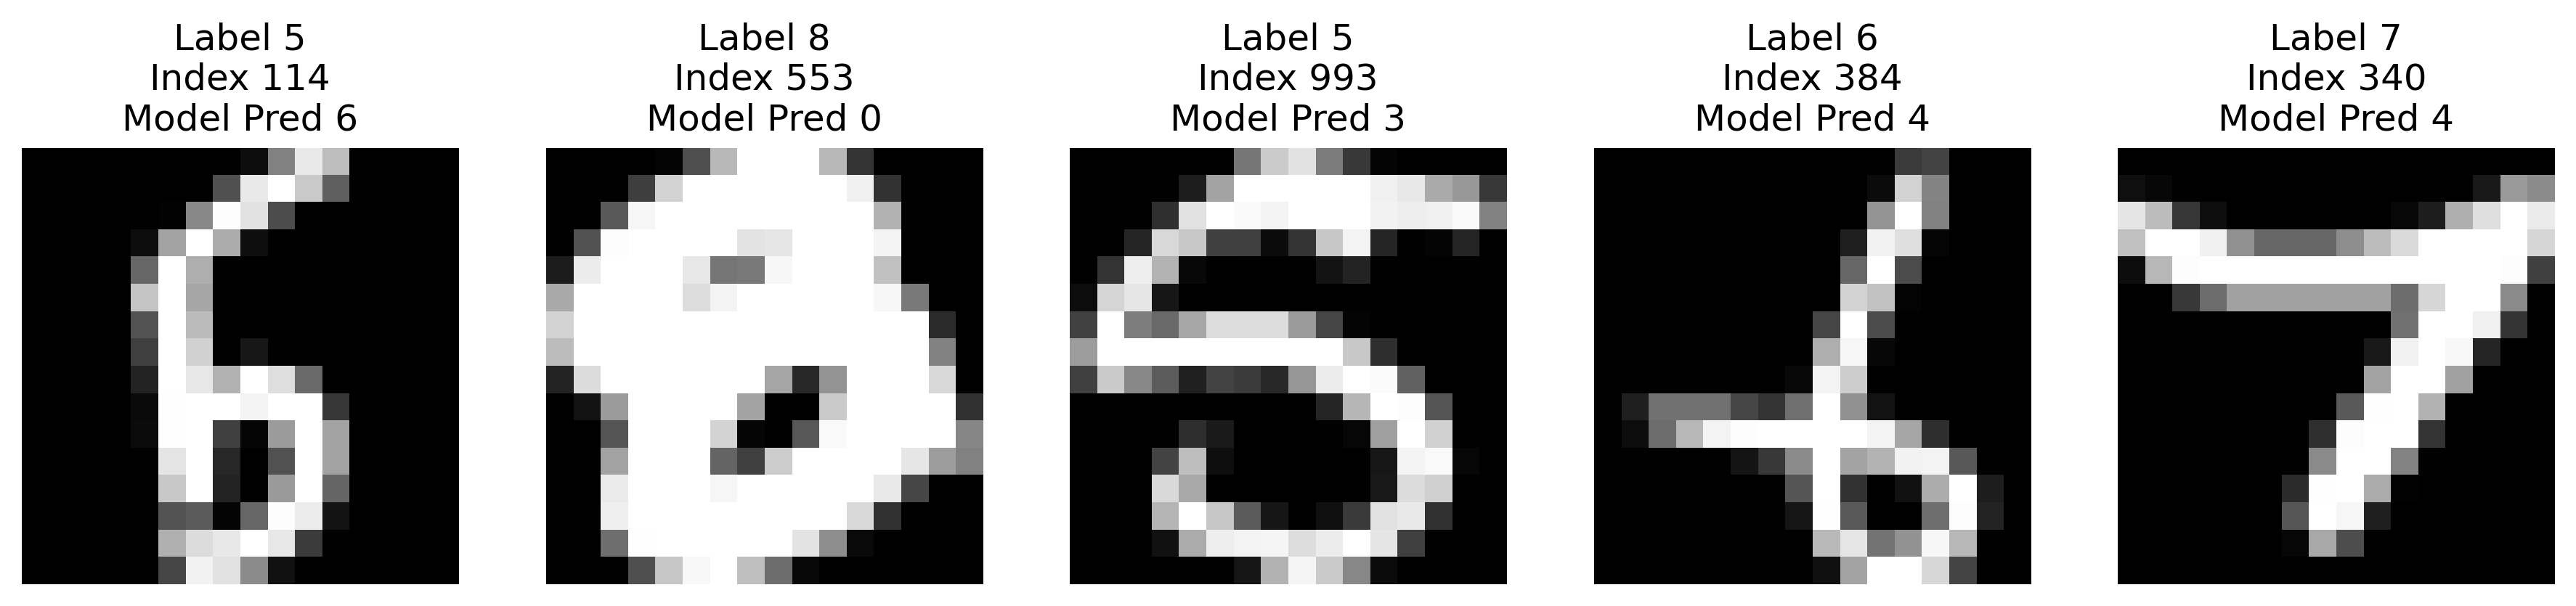
\includegraphics[width=0.7\textwidth]{outputs/figures/OvR_guass_Q6_hard_examples.png}
    \caption{}
    \label{fig:q1_poly_fits}
\end{figure}

\subsubsection{Comparison with Polynomial Kernel}
Overall the Gaussian kernel achieves slightly better test performance than the polynomial kernel. Using cross validation the gaussian kernel has a mean test error of $2.52\%$, compared to $2.71\%$ for the polynomial kernel.

The Gaussian kernel also has very low training error, this indicates a that the model fits the training data very well. However, its performance is sensitive to the choice of parameter $c$ with very large or small values leading to poorer generalisation.

Also note that while the gaussian kernel shows slight improvement in test accuracy, this comes at the cost of increased computation.



\subsection{One vs One}
The One vs One method provides an alternative strategy for extending a two class classifier to a k class classifier. Instead of training one sub-model per class against all other classes, the OvO method trains a submodel for every pair of classes, ie each sub model learns the classify between class $a$ and class $b$ only, it does not learn on any other classes. For $k$ classes this results in $\frac{k(k-1)}{2}$ binary classifiers, each specialised in distinguishing between a specific pair of classes.

At prediction time, each binary classifier votes for one of its two classes. The final predicted label is obtained by majority voting across all pairwise classifiers. Compared to the One vs Rest method, OvO has an increased computational cost due to the larger number of classifiers.

\subsubsection{One vs One Kernel Perceptron Implementation}
\begin{algorithm}[H]
\caption{One-vs-One Online Kernel Perceptron}
\begin{algorithmic}[1]

\STATE \textbf{Input:} $\{(x_i,y_i)\}_{i=1}^m$, classes $C=\{1,\dots,K\}$, kernel $K(\cdot,\cdot)$, epochs $T$
\STATE \textbf{Initialise:} For all $(a,b)$ with $a>b$,
$\alpha^{(a,b)}=\emptyset$, $I^{(a,b)}=\emptyset$

\FOR{$t=1,\dots,T$}
    \FOR{$i=1,\dots,m$}
        \STATE Initialise votes $v_k=0$
        \FOR{each pair $(a,b)$}
            \STATE $s_{a,b}(x_i)=\sum_{j\in I^{(a,b)}} \alpha^{(a,b)}_j K(x_j,x_i)$
            \STATE $v_a \leftarrow v_a + \mathbb{I}[s_{a,b}(x_i)\ge 0]$
            \STATE $v_b \leftarrow v_b + \mathbb{I}[s_{a,b}(x_i)<0]$
        \ENDFOR
        \STATE Predict $\hat y=\arg\max_k v_k$ \quad {(vote based)}
        \FOR{each pair $(a,b)$ with $y_i \in \{a,b\}$}
            \STATE
            $
            y_i^{(a,b)} =
            \begin{cases}
            +1 & \text{if } y_i = a \\
            -1 & \text{otherwise}
            \end{cases}
            $
            \IF{$\mathrm{sign}(s_{a,b}(x_i)) \neq y_i^{(a,b)}$}
                \STATE $I^{(a,b)} \leftarrow I^{(a,b)} \cup \{i\}$
                \STATE $\alpha^{(a,b)} \leftarrow \alpha^{(a,b)} \cup y_i^{(a,b)}$
            \ENDIF
        \ENDFOR
    \ENDFOR
\ENDFOR

\end{algorithmic}
\end{algorithm}



\subsection{One vs One : Polynomial Kernel Perceptron}
\subsubsection{Basic Results}
\begin{table}[H]
    \centering
    \begin{tabular}{rll}
\toprule
d & mean train error rates (\%) & mean test error rates (\%) \\
\midrule
1 & 0.167 $\pm$ 0.094 & 0.323 $\pm$ 0.493 \\
2 & 0.047 $\pm$ 0.023 & 0.376 $\pm$ 0.615 \\
3 & 0.044 $\pm$ 0.026 & 0.484 $\pm$ 0.634 \\
4 & 0.041 $\pm$ 0.026 & 0.645 $\pm$ 0.713 \\
5 & 0.041 $\pm$ 0.02 & 0.376 $\pm$ 0.615 \\
6 & 0.036 $\pm$ 0.022 & 0.43 $\pm$ 0.627 \\
7 & 0.025 $\pm$ 0.025 & 0.538 $\pm$ 0.721 \\
\bottomrule
\end{tabular}

    \caption{}
    \label{tab:q2_mse}
\end{table}
From the results above we observe the training errors decrease as the degree of the polynomial increases. We also observe expected U shape in test errors, as the value of $d$ decreases the test errors initially decrease up until the point $d = 5$, after which decreasing $d$ further causes test errors to increase as the model is overfitting to noise.

We conclude that the optimal parameter is $d = 5$
\subsubsection{Cross validation}
\begin{table}[H]
    \centering
    \begin{tabular}{rrr}
\toprule
run & d* & test error rate (\%) \\
\midrule
1 & 1.0000 & 0.2703 \\
2 & 1.0000 & 0.2703 \\
3 & 1.0000 & 0.8072 \\
4 & 4.0000 & 0.2703 \\
5 & 1.0000 & 0.2703 \\
6 & 1.0000 & 0.0000 \\
7 & 1.0000 & 0.2703 \\
8 & 1.0000 & 0.2703 \\
9 & 2.0000 & 0.8072 \\
10 & 1.0000 & 0.2703 \\
11 & 1.0000 & 0.0000 \\
12 & 2.0000 & 0.2703 \\
13 & 1.0000 & 0.2667 \\
14 & 6.0000 & 0.2703 \\
15 & 3.0000 & 0.2703 \\
16 & 1.0000 & 0.5369 \\
17 & 2.0000 & 0.2703 \\
18 & 7.0000 & 0.2667 \\
19 & 2.0000 & 0.2667 \\
20 & 1.0000 & 0.2703 \\
\bottomrule
\end{tabular}

    \caption{}
    \label{tab:q2_mse}
\end{table}
The results show that the optimal parameter has mean of 4.45±0.86458, train errors have a mean of 0.115±0.099\% and test errors have a mean of 3.2796±0.5049\%.
This aligns with the previous results without cross-validation where we identified the optimal parameter as being $d=5$
\subsubsection{Confusion Matrix}
\begin{table}[H]
    \centering
    \resizebox{\textwidth}{!}{%
        \begingroup
\scriptsize
\setlength{\tabcolsep}{3pt}
\begin{tabular}{lllllllllll}
\toprule
 & \textbf{0} & \textbf{1} & \textbf{2} & \textbf{3} & \textbf{4} & \textbf{5} & \textbf{6} & \textbf{7} & \textbf{8} & \textbf{9} \\
  &  &  &  &  &  &  &  &  &  &  \\
\midrule
0 & 0.000 ± 0.000 & 0.000 ± 0.000 & 0.000 ± 0.000 & 0.000 ± 0.000 & 0.000 ± 0.000 & 0.000 ± 0.000 & 0.000 ± 0.000 & 0.000 ± 0.000 & 0.000 ± 0.000 & 0.000 ± 0.000 \\
1 & 1.082 ± 2.629 & 0.000 ± 0.000 & 0.000 ± 0.000 & 0.000 ± 0.000 & 0.000 ± 0.000 & 0.000 ± 0.000 & 0.000 ± 0.000 & 0.000 ± 0.000 & 0.000 ± 0.000 & 0.000 ± 0.000 \\
2 & 0.000 ± 0.000 & 0.000 ± 0.000 & 0.000 ± 0.000 & 0.000 ± 0.000 & 0.000 ± 0.000 & 0.000 ± 0.000 & 0.000 ± 0.000 & 0.000 ± 0.000 & 0.000 ± 0.000 & 0.000 ± 0.000 \\
3 & 0.000 ± 0.000 & 0.000 ± 0.000 & 0.000 ± 0.000 & 0.000 ± 0.000 & 0.000 ± 0.000 & 0.000 ± 0.000 & 0.000 ± 0.000 & 0.000 ± 0.000 & 0.000 ± 0.000 & 0.000 ± 0.000 \\
4 & 0.000 ± 0.000 & 0.000 ± 0.000 & 0.000 ± 0.000 & 0.000 ± 0.000 & 0.000 ± 0.000 & 0.000 ± 0.000 & 0.000 ± 0.000 & 0.000 ± 0.000 & 0.000 ± 0.000 & 0.000 ± 0.000 \\
5 & 0.000 ± 0.000 & 0.625 ± 2.724 & 0.000 ± 0.000 & 0.000 ± 0.000 & 0.000 ± 0.000 & 0.000 ± 0.000 & 0.000 ± 0.000 & 0.000 ± 0.000 & 0.000 ± 0.000 & 0.000 ± 0.000 \\
6 & 0.000 ± 0.000 & 0.000 ± 0.000 & 0.000 ± 0.000 & 0.000 ± 0.000 & 0.000 ± 0.000 & 0.000 ± 0.000 & 0.000 ± 0.000 & 0.000 ± 0.000 & 0.000 ± 0.000 & 0.000 ± 0.000 \\
7 & 0.714 ± 3.113 & 0.000 ± 0.000 & 0.000 ± 0.000 & 0.000 ± 0.000 & 0.000 ± 0.000 & 0.000 ± 0.000 & 0.000 ± 0.000 & 0.000 ± 0.000 & 0.000 ± 0.000 & 0.000 ± 0.000 \\
8 & 0.000 ± 0.000 & 1.667 ± 7.265 & 0.000 ± 0.000 & 0.000 ± 0.000 & 0.000 ± 0.000 & 0.000 ± 0.000 & 0.000 ± 0.000 & 0.000 ± 0.000 & 0.000 ± 0.000 & 0.000 ± 0.000 \\
9 & 0.000 ± 0.000 & 0.000 ± 0.000 & 0.000 ± 0.000 & 0.000 ± 0.000 & 0.000 ± 0.000 & 0.000 ± 0.000 & 0.000 ± 0.000 & 0.000 ± 0.000 & 0.000 ± 0.000 & 0.000 ± 0.000 \\
\bottomrule
\end{tabular}

\endgroup

    }
    \caption{}
    \label{tab:q5_confusion}
\end{table}

\subsubsection{Hard to Predict Samples}
\begin{figure}[H]
    \centering
    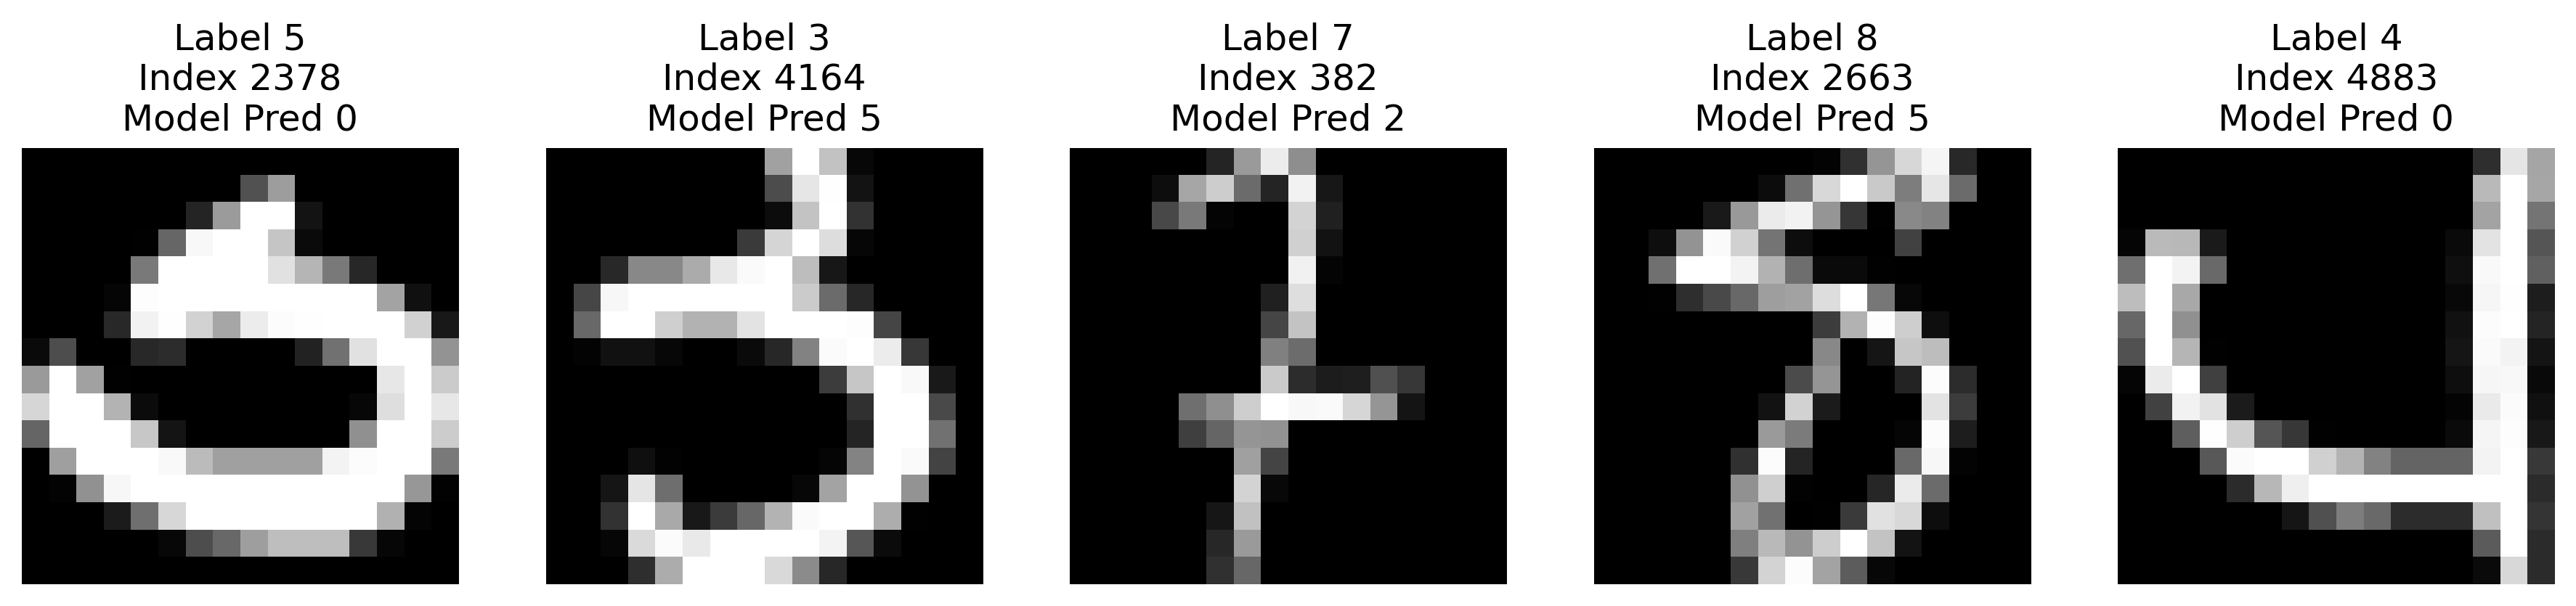
\includegraphics[width=0.7\textwidth]{outputs/figures/OvO_poly_Q6_hard_examples.png}
    \caption{}
    \label{fig:q1_poly_fits}
\end{figure}

\subsubsection{Comparison with One-vs-Rest}
Comparing the One vs One and One vs Rest method using the polynomial kernel, OvO achieves slightly worse test performance overall. OvR has a mean test error of $2.71\%$, compared to $3.28\%$ for OvO after cross validation. Additionally OvO is far more computationally expensive compared to OvR and as such for this dataset OvR would be the preferably method.

\end{document}